\documentclass[
  a4paper,
  oneside,
  BCOR = 10mm,
  DIV = 12,
  12pt,
  headings = normal,
]{scrartcl}

%%% Length calculations
\usepackage{calc}
%%%

%%% Support for color
\usepackage{xcolor}
\definecolor{lightblue}{HTML}{03A9F4}
\definecolor{red}{HTML}{F44336}
%%%

%%% Including graphics
\usepackage{graphicx}
%%%

%%% Font selection
\usepackage{fontspec}

\setromanfont{STIX Two Text}[
  SmallCapsFeatures = {LetterSpace = 8},
]

\setsansfont{IBM Plex Sans}[
  Scale = MatchUppercase,
]

\setmonofont{IBM Plex Mono}[
  Scale = MatchUppercase,
]
%%%

%%% Math typesetting
\usepackage{amsmath}

\usepackage{unicode-math}
\setmathfont{STIX Two Math}

\usepackage{IEEEtrantools}
%%%

%%% List settings
\usepackage{enumitem}
\setlist[enumerate]{
  label*      = {\arabic*.},
  left        = \parindent,
  topsep      = 0\baselineskip,
  parsep      = 0\baselineskip,
  noitemsep, % override itemsep
}
% List settings for levels 2–4
\setlist[enumerate, 2, 3, 4]{
  label*      = {\arabic*.},
  left        = 0em,
  topsep      = 0\baselineskip,
  parsep      = 0\baselineskip,
  noitemsep, % override itemsep
}

\setlist[itemize]{
  label*      = {—},
  left        = \parindent,
  topsep      = 0\baselineskip,
  parsep      = 0\baselineskip,
  itemsep     = 1\baselineskip,
  noitemsep, % override itemsep
}

\setlist[description]{
  font        = {\rmfamily\upshape\bfseries},
  topsep      = 1\baselineskip,
  parsep      = 0\baselineskip,
  itemsep     = 0\baselineskip,
}

%%%

%%% Structural elements typesetting
\setkomafont{pagenumber}{\rmfamily\upshape}
\setkomafont{disposition}{\rmfamily\bfseries}

% Sectioning
\RedeclareSectionCommand[
  beforeskip = -1\baselineskip,
  afterskip  = 1\baselineskip,
  font       = {\normalsize\bfseries\scshape},
]{section}

\RedeclareSectionCommand[
  beforeskip = -1\baselineskip,
  afterskip  = 1\baselineskip,
  font       = {\normalsize\bfseries\itshape},
]{subsection}

\RedeclareSectionCommand[
  beforeskip = -1\baselineskip,
  afterskip  = 1\baselineskip,
  font       = {\normalsize\bfseries},
]{subsubsection}

\RedeclareSectionCommand[
  beforeskip = -1\baselineskip,
  afterskip  = -0.5em,
  font       = {\normalsize\mdseries\scshape\addfontfeatures{Letters = {UppercaseSmallCaps}}},
]{paragraph}
%%%

%%% Typographic enhancements
\usepackage{microtype}
%%%

%%% Language-specific settings
\usepackage{polyglossia}
\setmainlanguage{ukrainian}
\setotherlanguages{english}
%%%

%%% Captions
\usepackage{caption}
\usepackage{subcaption}

%\DeclareCaptionLabelFormat{closing}{#2)}
%\captionsetup[subtable]{labelformat = closing}

%\captionsetup[subfigure]{labelformat = closing}

\captionsetup[table]{
  aboveskip = 0\baselineskip,
  belowskip = 0\baselineskip,
}

\captionsetup[figure]{
  aboveskip = 1\baselineskip,
  belowskip = 0\baselineskip,
}

\captionsetup[subfigure]{
  labelformat = simple,
  labelformat = brace,
  justification = RaggedRight,
  singlelinecheck = false,
}
%%%

%%% Hyphenated ragged typesetting
\usepackage{ragged2e}
%%%

%%% Table typesetting
\usepackage{booktabs}
\usepackage{longtable}

\usepackage{multirow}

\usepackage{array}
\newcolumntype{v}[1]{>{\RaggedRight\arraybackslash\hspace{0pt}}p{#1}}
\newcolumntype{b}[1]{>{\Centering\arraybackslash\hspace{0pt}}p{#1}}
\newcolumntype{n}[1]{>{\RaggedLeft\arraybackslash\hspace{0pt}}p{#1}}
%%%

%%% Drawing
\usepackage{tikz}
\usepackage{tikzscale}
\usetikzlibrary{datavisualization}
\usetikzlibrary{datavisualization.formats.functions}
\usetikzlibrary{positioning}
\usetikzlibrary{patterns}
\usetikzlibrary{intersections}
\usetikzlibrary{arrows.meta} % Stealth arrow tips
\usetikzlibrary{graphs}
\usetikzlibrary{graphdrawing}
\usegdlibrary{trees}
\usetikzlibrary{quotes}

\usepackage{pgfplots}
\usepgfplotslibrary{fillbetween}
%%%

%%% SI units typesetting
\usepackage{siunitx}
\sisetup{
  output-decimal-marker = {,},
  exponent-product      = {\cdot},
  inter-unit-product    = \ensuremath{{} \cdot {}},
  per-mode              = symbol,
}
%%%

% Code Highlighting
\usepackage{minted}
\setmintedinline{
  style = bw,
  breaklines,
}

\newminted[bashterm]{text}{%
  autogobble,%
  breaklines,%
  style=bw,%
}

\newminted[codegeneric]{text}{%
  autogobble,%
  style=bw,%
  breaklines,%
  fontsize=\small,%
}

\newmintinline{bash}{%
}

\newmintinline[minttext]{text}{%
  breaklines,%
  breakanywhere,%
}

%%% Framing code listings
\usepackage{tcolorbox}
\tcbuselibrary{breakable}
\tcbuselibrary{minted}
\tcbuselibrary{skins}

% Text file listing
\newtcblisting[
  auto counter,
  list inside,
  number within = section,
]{listingplaintext}[3][]{%
  minted language = text,
  minted style    = bw,
  minted options  = {
    autogobble,
    linenos,
    tabsize = 4,
    breaklines,
    breakanywhere,
    fontsize = \footnotesize,
  },
  empty,
  sharp corners,
  coltitle = black,
  borderline horizontal = {1pt}{0pt}{black},
  titlerule = {0.5pt},
  titlerule style = {
    black,
  },
  toptitle = 0.3em,
  bottomtitle = 0.3em,
  before skip      = \intextsep,
  after  skip      = \intextsep,
  title            = {Лістинг \thetcbcounter: #2},
  list entry       = {\protect\numberline{\thetcbcounter}#2},
  left = 0em,
  right = 0em,
  %
  listing only,
  breakable,
  %
  label = {#3},%
}

\newtcbinputlisting[
  use counter from = listingplaintext,
  list inside,
  number within = section
]{\inputplaintext}[4][]{%
  minted language = text,
  minted style    = bw,
  minted options  = {
    autogobble,
    linenos,
    tabsize = 4,
    breaklines,
    breakanywhere,
    fontsize = \footnotesize,
  },
  empty,
  sharp corners,
  coltitle = black,
  borderline horizontal = {1pt}{0pt}{black},
  titlerule = {0.5pt},
  titlerule style = {
    black,
  },
  toptitle = 0.3em,
  bottomtitle = 0.3em,
  before skip      = \intextsep,
  after  skip      = \intextsep,
  title            = {Лістинг \thetcbcounter: #3},
  list entry       = {\protect\numberline{\thetcbcounter}#3},
  left = 0em,
  right = 0em,
  %
  listing file={#2},
  listing only,
  breakable,
  %
  label = {#4}
}

\newtcblisting[
  use counter from = listingplaintext,
  list inside,
  number within = section,
]{listingpython}[3][]{%
  minted language = python,
  minted style    = bw,
  minted options  = {
    autogobble,
    linenos,
    tabsize = 4,
    breaklines,
    breakanywhere,
    fontsize = \footnotesize,
  },
  empty,
  sharp corners,
  coltitle = black,
  borderline horizontal = {1pt}{0pt}{black},
  titlerule = {0.5pt},
  titlerule style = {
    black,
  },
  toptitle = 0.3em,
  bottomtitle = 0.3em,
  before skip      = \intextsep,
  after  skip      = \intextsep,
  title            = {Лістинг \thetcbcounter: #2},
  list entry       = {\protect\numberline{\thetcbcounter}#2},
  left = 0em,
  right = 0em,
  %
  listing only,
  breakable,
  %
  label = {#3},
  %
  #1%
}

\newtcbinputlisting[
  use counter from = listingplaintext,
  list inside,
  number within = section
]{\inputpython}[4][]{%
  minted language = python,
  minted style    = bw,
  minted options  = {
    autogobble,
    linenos,
    tabsize = 4,
    breaklines,
    breakanywhere,
    fontsize = \footnotesize,
  },
  empty,
  sharp corners,
  coltitle = black,
  borderline horizontal = {1pt}{0pt}{black},
  titlerule = {0.5pt},
  titlerule style = {
    black,
  },
  toptitle = 0.3em,
  bottomtitle = 0.3em,
  before skip      = \intextsep,
  after  skip      = \intextsep,
  title            = {Лістинг \thetcbcounter: #3},
  list entry       = {\protect\numberline{\thetcbcounter}#3},
  left = 0em,
  right = 0em,
  %
  listing file={#2},
  listing only,
  breakable,
  %
  label = {#4}
}

% Linux command-line listing
\newtcblisting{linuxterm}%
{%
  % Syntax highlighing options
  listing only,%
  minted language = bash,%
  minted options={%
    autogobble,%
    linenos%
  },%
  % Presentation options
  empty,%
  %% Margins
  sharp corners,%
  toptitle = 0.0em,%
  bottomtitle = 0.0em,%
  left = 0em,%
  right = 0em,%
  before skip = \intextsep,%
  after skip = \intextsep,%
}

\newtcblisting{linuxtermout}%
{%
  % Syntax highlighing options
  listing only,%
  minted language = text,%
  minted options={%
    autogobble,%
    linenos%
  },%
  % Presentation options
  empty,%
  %% Margins
  sharp corners,%
  toptitle = 0.0em,%
  bottomtitle = 0.0em,%
  left = 0em,%
  right = 0em,%
  before skip = \intextsep,%
  after skip = \intextsep,%
}

% Dockerfile listings
\newtcblisting[
  use counter from = listingplaintext,
  list inside,
  number within = section,
]{listingdocker}[3][]{%
  minted language = dockerfile,
  minted style    = bw,
  minted options  = {
    autogobble,%
    linenos,
    tabsize = 4,
    breaklines,
    breakanywhere,
    fontsize = \footnotesize,
  },
  empty,
  sharp corners,
  coltitle = black,
  borderline horizontal = {1pt}{0pt}{black},
  titlerule = {0.5pt},
  titlerule style = {
    black,
  },
  toptitle = 0.3em,
  bottomtitle = 0.3em,
  before skip      = \intextsep,
  after  skip      = \intextsep,
  title            = {Лістинг \thetcbcounter: #2},
  list entry       = {\protect\numberline{\thetcbcounter}#2},
  left = 0em,
  right = 0em,
  %
  listing only,
  breakable,
  %
  label = {#3},%
}

% Docker Compose listings
\newtcblisting[
  use counter from = listingplaintext,
  list inside,
  number within = section,
]{listingdockercompose}[3][]{%
  minted language = yaml,
  minted style    = bw,
  minted options  = {
    autogobble,%
    linenos,
    tabsize = 4,
    breaklines,
    breakanywhere,
    fontsize = \footnotesize,
  },
  empty,
  sharp corners,
  coltitle = black,
  borderline horizontal = {1pt}{0pt}{black},
  titlerule = {0.5pt},
  titlerule style = {
    black,
  },
  toptitle = 0.3em,
  bottomtitle = 0.3em,
  before skip      = \intextsep,
  after  skip      = \intextsep,
  title            = {Лістинг \thetcbcounter: #2},
  list entry       = {\protect\numberline{\thetcbcounter}#2},
  left = 0em,
  right = 0em,
  %
  listing only,
  breakable,
  %
  label = {#3},%
}


% Customize minted line numbers
\renewcommand{\theFancyVerbLine}{\ttfamily\scriptsize\arabic{FancyVerbLine}}

%%%

%%% Typeset menus and keys
\usepackage{menukeys}[
  os=win,
]
%%%

%%% Links and hyperreferences
\usepackage{hyperref}
\hypersetup{
  bookmarksnumbered = true,
  colorlinks      = false,
  linkbordercolor = red,
  urlbordercolor  = lightblue,
  pdfborderstyle  = {/S/U/W 1.5},
}
%%%

%%% Length adjustment

% Set baselineskip, default is 14.5 pt
\linespread{1.068966} % ~15.5 pt
\setlength{\emergencystretch}{1em}
\setlength{\parindent}{1.5em}
\newlength{\gridunitwidth}
\setlength{\gridunitwidth}{\textwidth / 12}
%%%

%%% Custom commands
\newcommand{\allcaps}[1]{%
  {%
    \addfontfeatures{%
      Letters = UppercaseSmallCaps,
      LetterSpace = 8,%
    }%
    #1%
  }%
}
\newcommand{\filename}[1]{\texttt{#1}}
\newcommand{\progname}[1]{\texttt{#1}}
\newcommand{\commandname}[1]{\texttt{#1}}
\newcommand{\modulename}[1]{\texttt{#1}}
\newcommand{\transeng}[1]{{англ.}~\textit{\textenglish{#1}}}
%%%

%%% Custom math commands
\newcommand{\longvar}[1]{\mathit{#1}}
\newcommand{\vect}[1]{\mathbfit{#1}}
\newcommand{\matr}[1]{\mathbfit{#1}}

\newcommand{\logequiv}{\mathrel{\Longleftrightarrow}} % Logically equivalent

\DeclareMathOperator*{\minimize}{min} % minimize for linear programs
%%%

\begin{document}

\begin{titlepage}
    \begin{center}
      Міністерство освіти і~науки України\\
      Національний авіаційний університет\\
      Факультет кібербезпеки, комп'ютерної та~програмної інженерії\\
      Кафедра комп'ютеризованих систем управління

      \vspace{\fill}
        Лабораторна робота №~1.5\\
        з~дисципліни «Системи штучного інтелекту»\\
        на~тему «Моделі представлення знань»

      \vspace{\fill}

      \begin{flushright}
        Виконав:\\
        студент \allcaps{ФККПІ}\\
        групи \allcaps{СП}-425\\
        Клокун В.\,Д.\\
        Перевірила:\\
        Росінська Г.\,П.
      \end{flushright}

      Київ 2019
    \end{center}
  \end{titlepage}

  \section{Завдання роботи}
    Ознайомитись з~моделями представлення знань і~проаналізувати їх~реалізацію на~прикладі існуючих експертних систем.

  \section{Хід~роботи}
    \subsection{Симптомус}
      Щоб~виконати лабораторну роботу, переходимо на~сайт експертної системи~«Симптомус». Виявляється, що~вона закрита~(рис.~\ref{fig:simptomus}).

      \begin{figure}[!htbp]
        \centering
        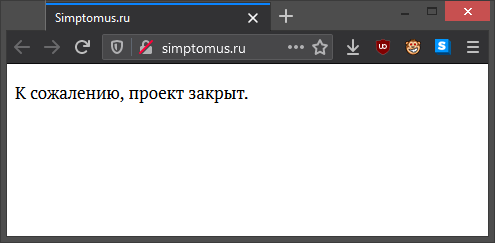
\includegraphics[width = 8 \gridunitwidth]{./assets/01.png}
        \caption{Веб-сторінка проекту «Симптомус»}
        \label{fig:simptomus}
      \end{figure}

    \subsection{Експертна медична система з~гомеопатії}
      Переходимо на~веб-сторінку експертної медичної системи з~гомеопатії~(рис.~\ref{fig:homeopathy}). Щоб~використати її, починаємо вводити симптоми. Для~того, щоб~система могла порадити препарат, необхідно ввести достатню кількість симптомів.

      \begin{figure}[!htbp]
        \begin{subfigure}[b]{6 \gridunitwidth - 1em /2}
          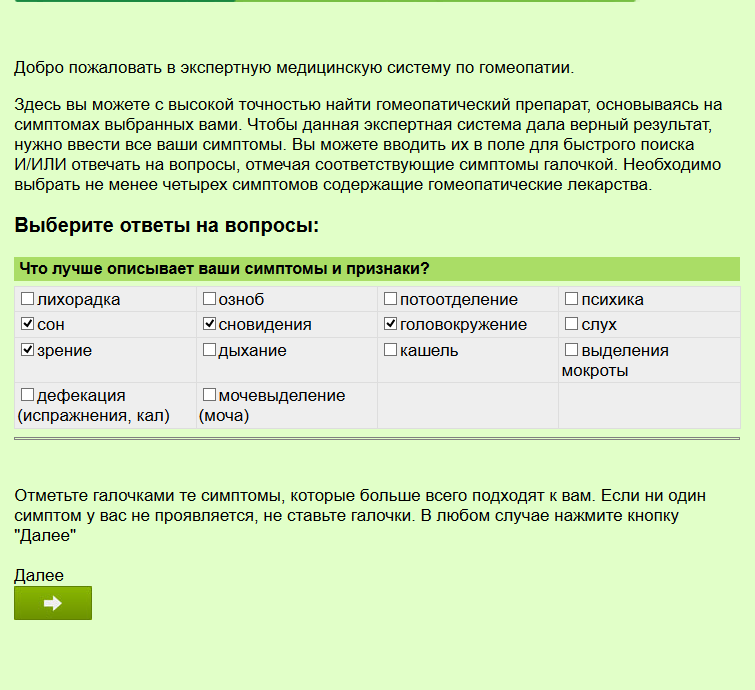
\includegraphics[width = \columnwidth]{./assets/02.png}
          \caption{}
          \label{subfig:homeopathy-01}
        \end{subfigure}%
        \hspace{1em}%
        \begin{subfigure}[b]{6 \gridunitwidth - 1em /2}
          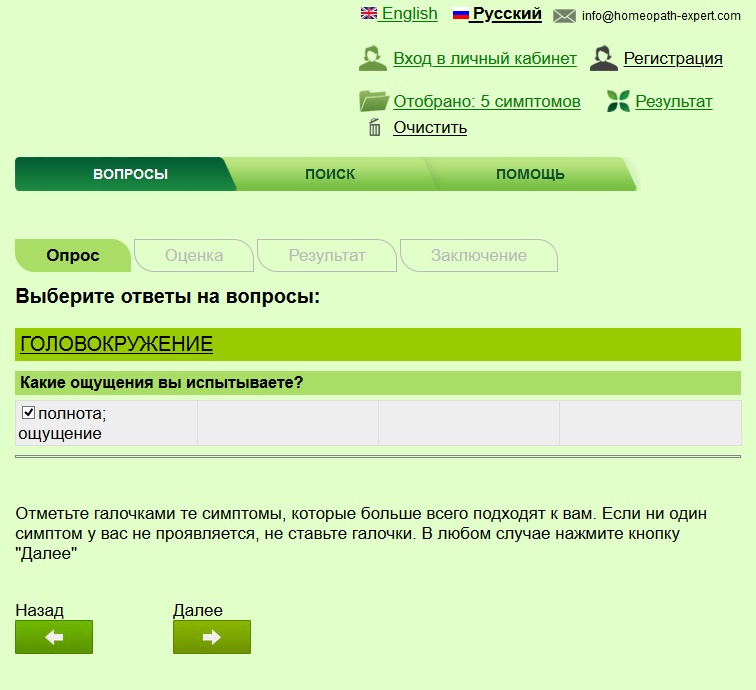
\includegraphics[width = \columnwidth]{./assets/03.png}
          \caption{}
          \label{subfig:homeopathy-02}
        \end{subfigure}
        \begin{subfigure}[b]{6 \gridunitwidth - 1em /2}
          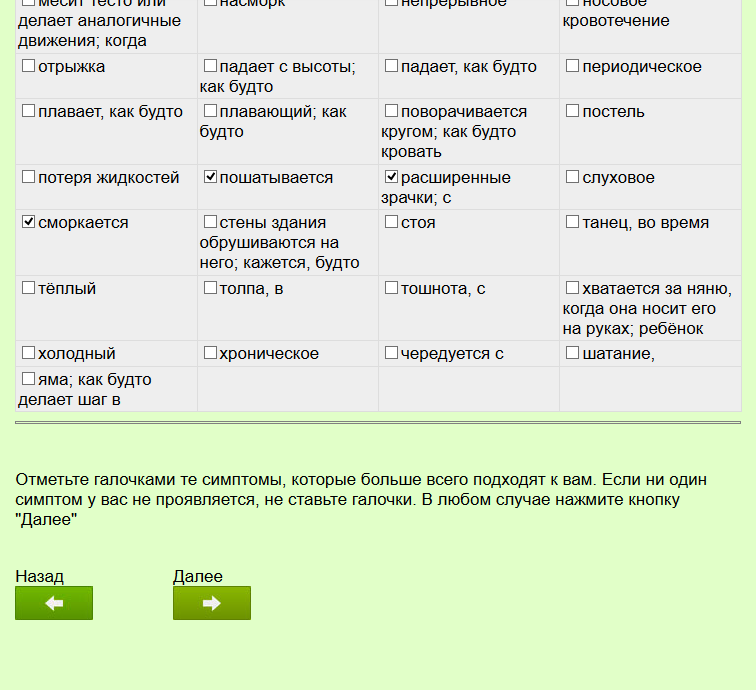
\includegraphics[width = \columnwidth]{./assets/04.png}
          \caption{}
          \label{subfig:homeopathy-03}
        \end{subfigure}%
        \hspace{1em}%
        \begin{subfigure}[b]{6 \gridunitwidth - 1em /2}
          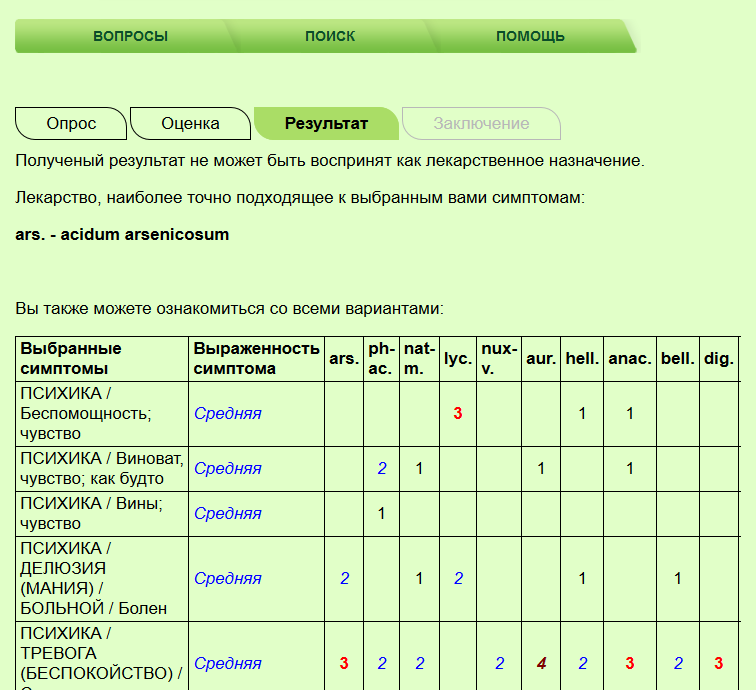
\includegraphics[width = \columnwidth]{./assets/05.png}
          \caption{}
          \label{subfig:homeopathy-04}
        \end{subfigure}%
        \caption{Експертна медична система з~гомеопатії}
        \label{fig:homeopathy}
      \end{figure}

    \subsection{Діагноз.ру}
      Переходимо на~веб-сайт системи постановки діагнозу за~симптомами «Діагноз.ру». Щоб~використати її, запускаємо опитування і~відповідаємо на~поставлені питання~(рис.~\ref{fig:diagnos-ru}).

      \begin{figure}[!htbp]
        \begin{subfigure}[b]{6 \gridunitwidth - 1em /2}
          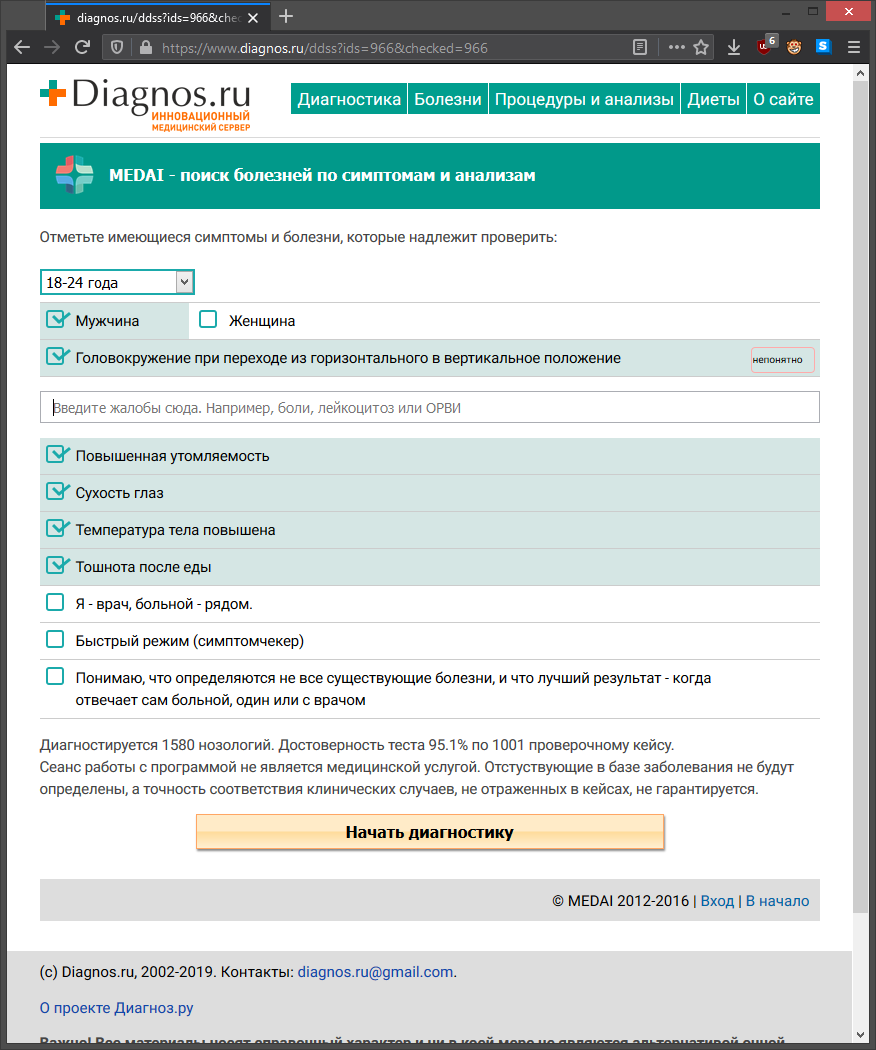
\includegraphics[width = \columnwidth]{./assets/06.png}
          \caption{}
          \label{subfig:diagnos-ru-01}
        \end{subfigure}%
        \hspace{1em}%
        \begin{subfigure}[b]{6 \gridunitwidth - 1em /2}
          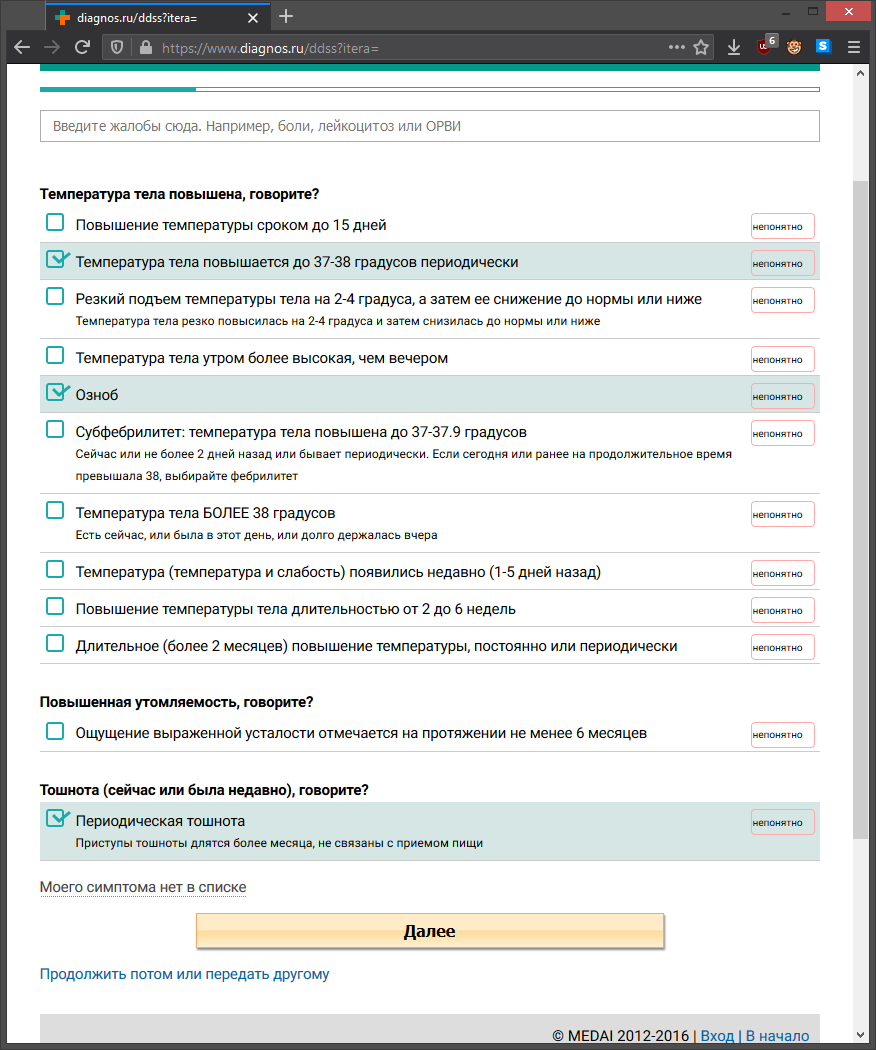
\includegraphics[width = \columnwidth]{./assets/07.png}
          \caption{}
          \label{subfig:diagnos-ru-02}
        \end{subfigure}
        \begin{subfigure}[b]{6 \gridunitwidth - 1em /2}
          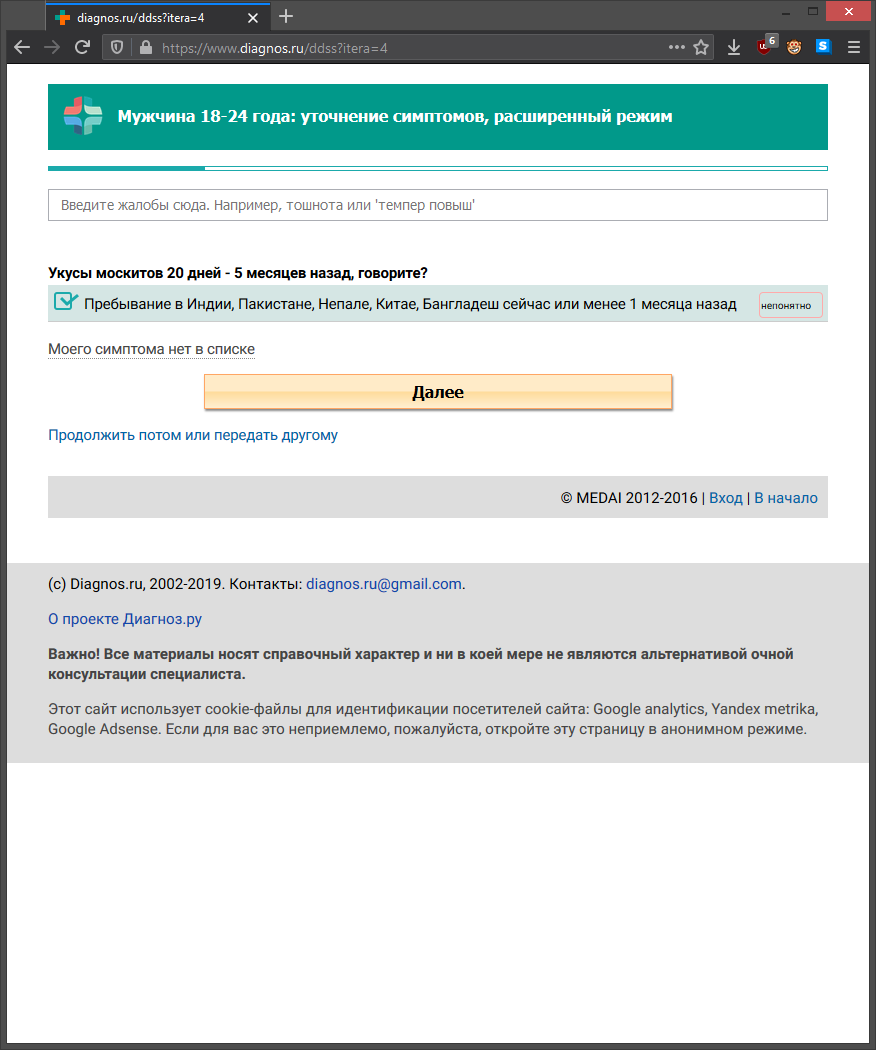
\includegraphics[width = \columnwidth]{./assets/09.png}
          \caption{}
          \label{subfig:diagnos-ru-03}
        \end{subfigure}%
        \hspace{1em}%
        \begin{subfigure}[b]{6 \gridunitwidth - 1em /2}
          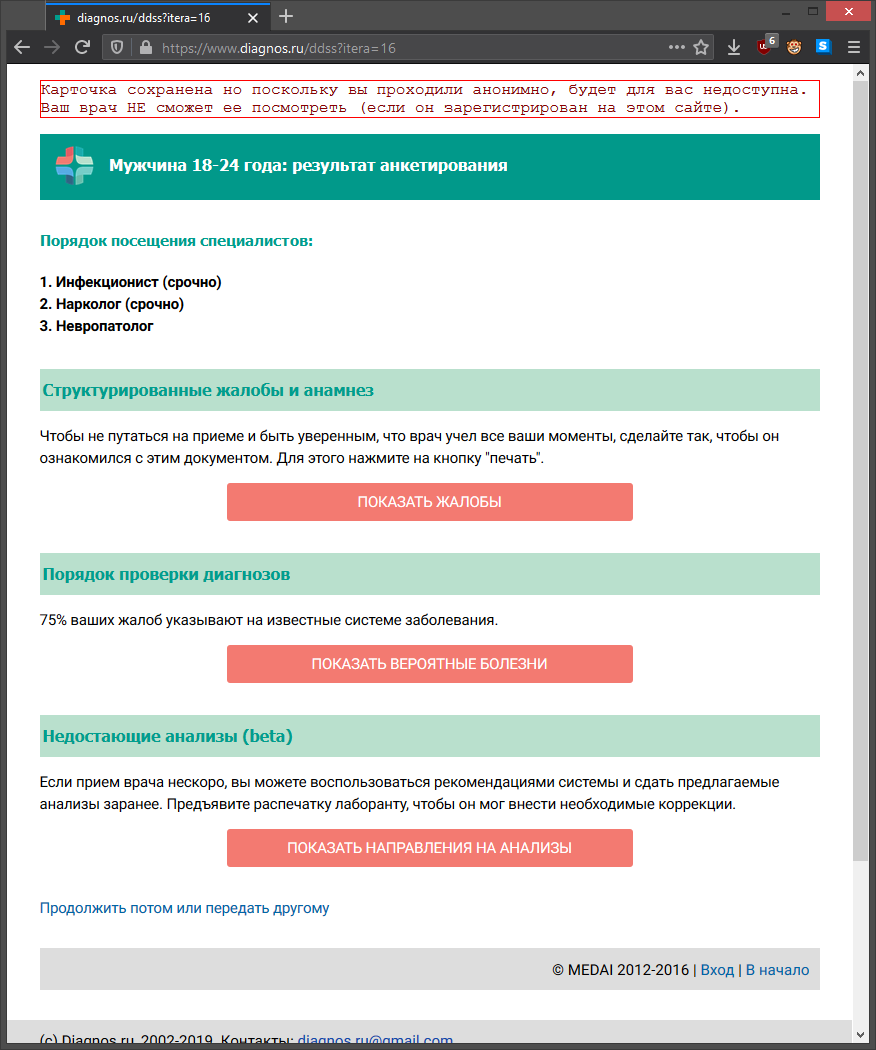
\includegraphics[width = \columnwidth]{./assets/10.png}
          \caption{}
          \label{subfig:diagnos-ru-04}
        \end{subfigure}%
        \caption{Експертна медична система «Діагноз.ру»}
        \label{fig:diagnos-ru}
      \end{figure}

    \subsection{\textenglish{WordNet}}
      Переходимо на~веб-сайт системи~«\textenglish{WordNet}». Щоб~використати її, вводимо слово і~спостерігаємо результат~— опис синонімів~(рис.~\ref{fig:wordnet}).

      \begin{figure}[!htbp]
        \centering
        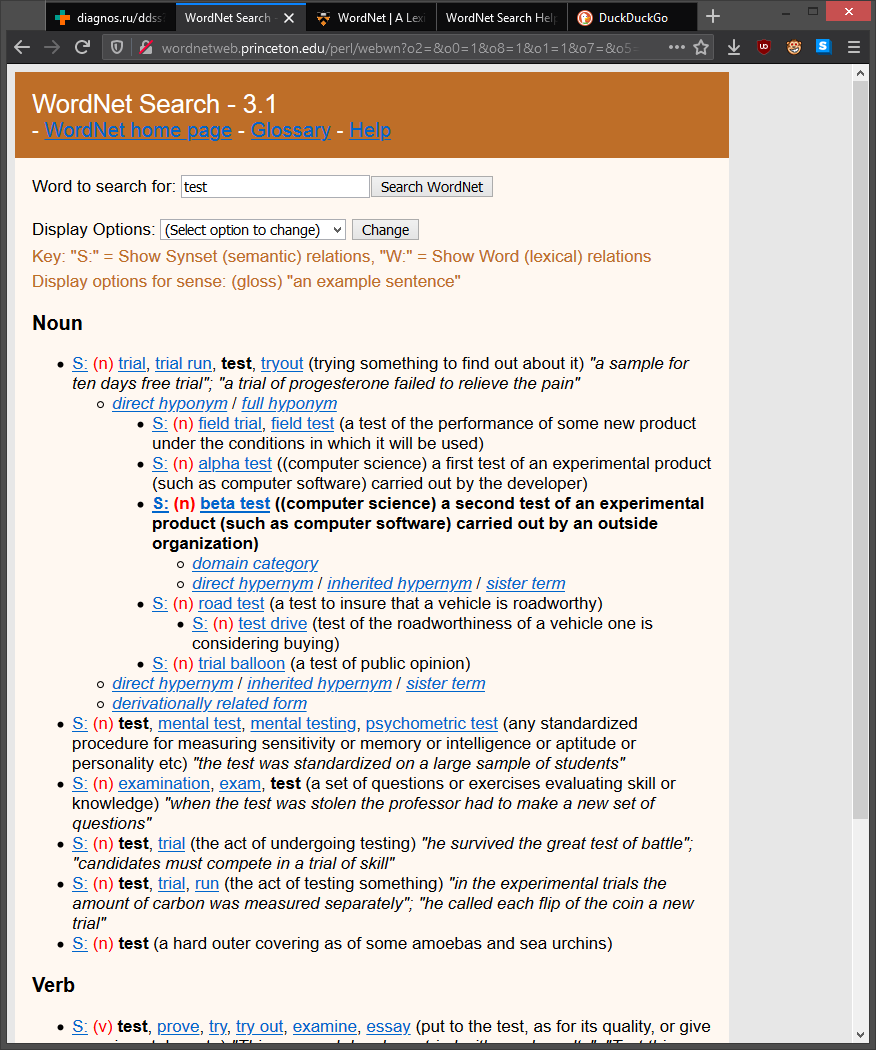
\includegraphics[width = 8 \gridunitwidth]{./assets/11.png}
        \caption{Результат пошуку слова у~«\textenglish{WordNet}»}
        \label{fig:wordnet}
      \end{figure}

    \subsection{«Акінатор»}
      Переходимо на~веб-сайт системи~«Акінатор». Щоб~використати її, запускаємо гру~і~відповідаємо на~поставлені питання~(рис.~\ref{fig:akinator}). Як~бачимо, «Акінатор» правильно визначив загаданого персонажа.

      \begin{figure}[!htbp]
        \begin{subfigure}[b]{6 \gridunitwidth - 1em /2}
          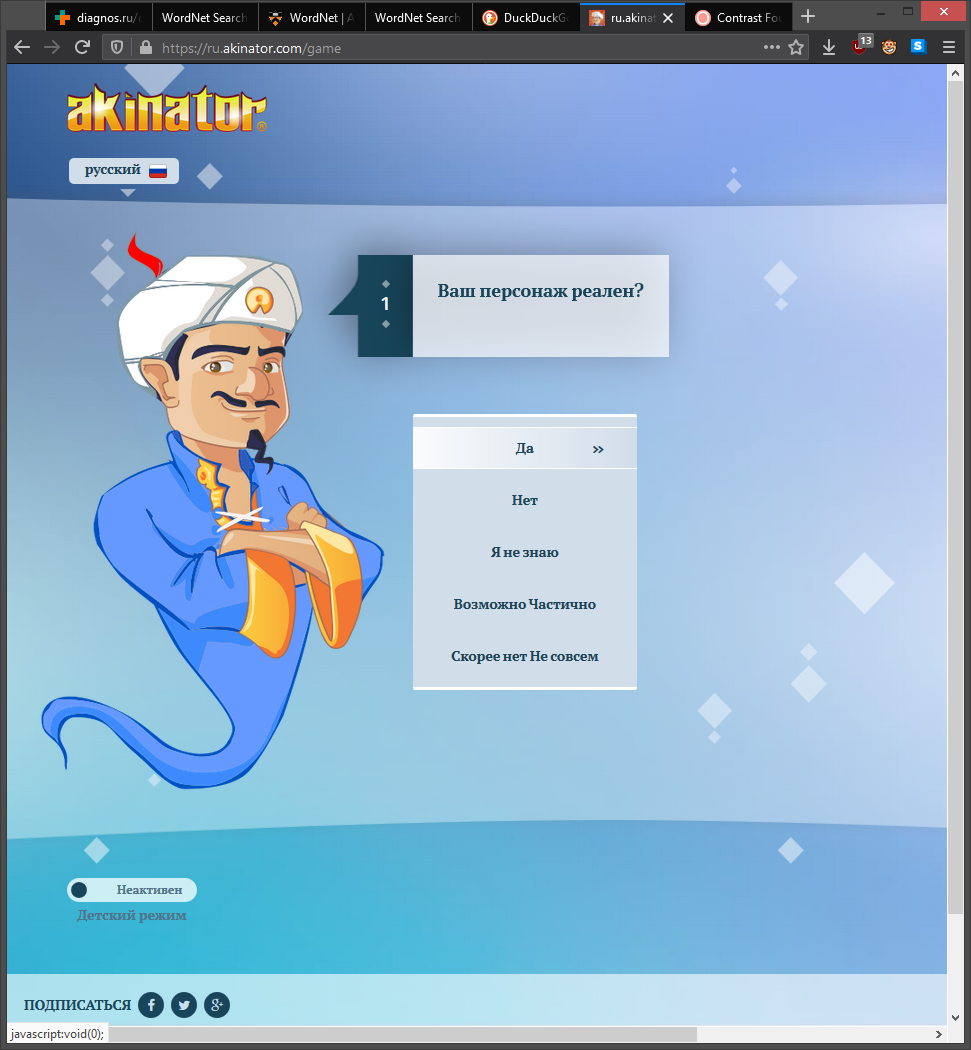
\includegraphics[width = \columnwidth]{./assets/12.png}
          \caption{}
          \label{subfig:akinator-01}
        \end{subfigure}%
        \hspace{1em}%
        \begin{subfigure}[b]{6 \gridunitwidth - 1em /2}
          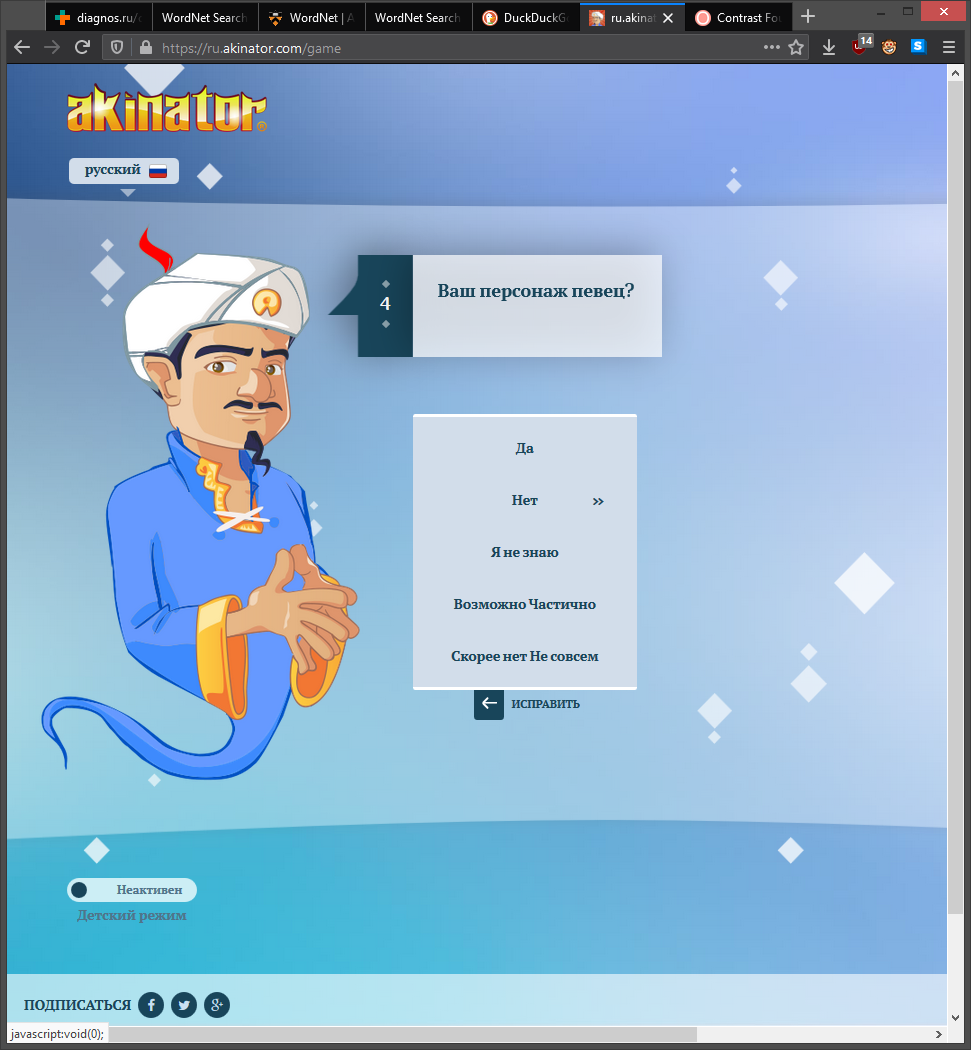
\includegraphics[width = \columnwidth]{./assets/13.png}
          \caption{}
          \label{subfig:akinator-02}
        \end{subfigure}
        \begin{subfigure}[b]{6 \gridunitwidth - 1em /2}
          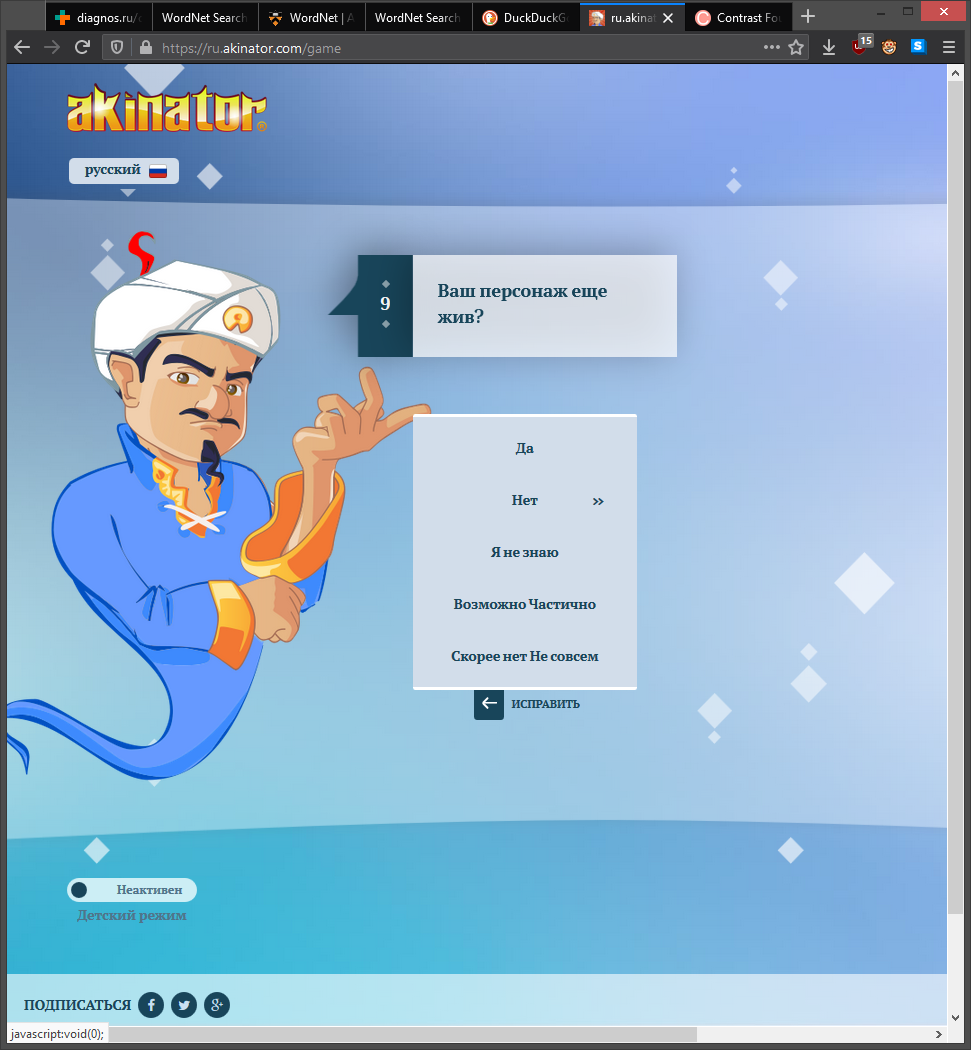
\includegraphics[width = \columnwidth]{./assets/14.png}
          \caption{}
          \label{subfig:akinator-03}
        \end{subfigure}%
        \hspace{1em}%
        \begin{subfigure}[b]{6 \gridunitwidth - 1em /2}
          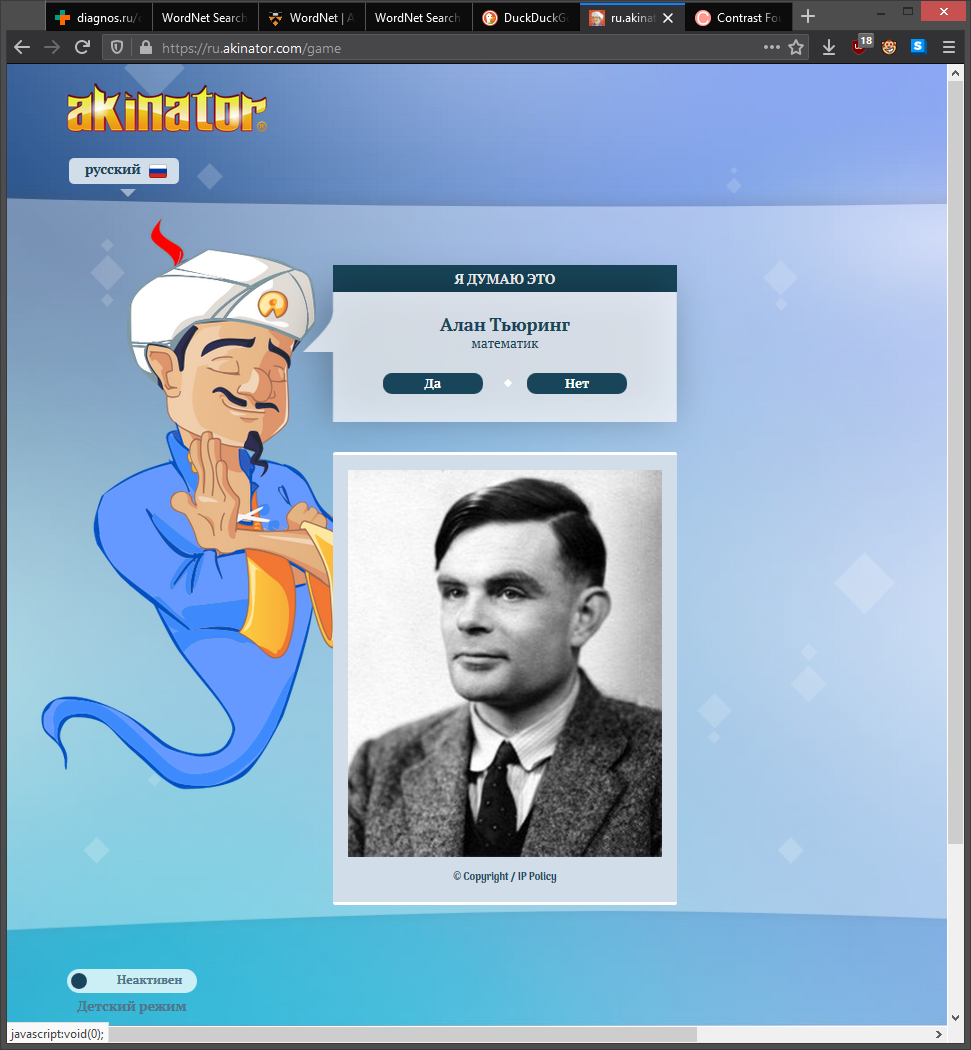
\includegraphics[width = \columnwidth]{./assets/15.png}
          \caption{}
          \label{subfig:akinator-04}
        \end{subfigure}%
        \caption{Результат роботи з~«Акінатором»}
        \label{fig:akinator}
      \end{figure}

  \section{Висновок}
    Під~час~виконання лабораторної роботи ми~досліджували експертні системи «Симптомус», «Експертна медична система з~гомеопатії», «Діагноз.ру», «\textenglish{WordNet}» і~«Акінатор». Система «Симптомус» була недоступна. «Експертна медична система з~гомеопатії» запрошувала визначати симптоми до~тих~пір, поки користувач не~вирішить, що~він~обрав достатню кількість симптомів. Коли користувач просить показати йому результат, система виводить обраний препарат після десяти симптомів, досить невеликої кількості вхідної інформації.

    Система «Діагноз.ру» працює за~аналогічним принципом: вона задає питання, аналізує відповіді, задає уточнюючі питання на~основі отриманих відповідей і~продовжує так~доти, доки не~отримає достатню кількість інформації. Під~час~виконання лабораторної роботи знадобилось близько 100~відповідей, щоб~отримати результат.

    Система «\textenglish{WordNet}» дозволяє шукати та~визначати синоніми до~шуканого слова, а~також переглядати причини, чому вона так~вважає: переглянути прямий або~повний гіпоніми, переглянути сінсет синоніма тощо.

    Система «Акінатор» намагається вгадати, якого персонажа загадав користувач. Як~і~медичні експертні системи, вона задає питання і~на~основі отриманих відповідей задає уточнюючі питання, щоб~із~більшою імовірністю вгадати персонажа. Система «Акінатор» вже~довго працює, тому має~велику базу знань, і~тому прекрасно вгадує відомих і~наразі популярних персонажей, буквально за~декілька кроків.

    Виконуючи дану лабораторну роботу, ми~ознайомились з~моделями представлення знань і~проаналізували їх~реалізацію на~прикладі існуючих експертних систем.

\end{document}
